\documentclass{article} 
\usepackage{geometry}
\geometry{legalpaper, portrait, margin=1in}
\usepackage{fancyhdr}
\usepackage{enumerate}
\usepackage{listings}
\usepackage{amsmath}
\usepackage{algorithm}
\usepackage{algpseudocode}
\usepackage{graphicx}
\usepackage{hyperref}
\graphicspath{ }

\title{OpenFlow-based Adaptive Routing for Wireless Networks}
\author{
    Alok Kulkarni \\
    \textit{akulkar4@ncsu.edu}
    \and
    Angelyn Arputha Babu John \\
    \textit{ababujo@ncsu.edu}
    \and
    Jignesh Darji \\
    \textit{jndarji@ncsu.edu}
    \and 
    Nishad Sabnis \\
    \textit{nsabnis@ncsu.edu}
}
\date{
    \small{\url{https://sites.google.com/a/ncsu.edu/openflow-based-adaptive-routing-for-wireless-networks}}\\
    October 4th, 2015}

\pagestyle{fancy}
\fancyhf{}
\rhead{OpenFlow-based Adaptive Routing for Wireless Networks}
\lhead{CSC573}
\rfoot{Page \thepage}
\begin{document}
\maketitle
\section{Introduction}
\subsection{Problem Statement}
Designing a system to enable adaptive routing in a wireless network in order to make a comparative analysis of the
throughput efficiency of ground nodes versus aerial nodes.
\subsection{Problem Description}
\par We aim to implement OpenFlow based adaptive routing in an ad-hoc network by monitoring the link quality between wireless
nodes. We anticipate that in such a network which offers multiple wireless routes between two end-points, the
fluctuations in the RF link qualities between the endpoints will play an important role in determining the best end to
end path. Determining the wireless link quality between each and every inter-connected node and making routing decisions
based on this information constitute the two major parts of the problem. 
\par We plan to make aerial nodes a part of the network which will be used for testing. Aerial nodes have their own set of
advantages and disadvantages. They are less susceptible to electromagnetic interferences and can beam wifi over a large
area if the antennae are powerful enough. However, the number of aerial nodes and naturally the number of available
links through such nodes is likely to be lesser due to the low prevalence of such nodes. These trade offs need to be
accounted for while making the routing decisions as well. The final aim is to ensure that the flow tables are
dynamically modified to ensure effective end to end packet transmission. 
\section{Components}
\subsection{Platforms for the project}
\begin{itemize}
\item CentMesh
\item OpenFlow v1.3
\item OpenDaylight
\item Ubuntu
\end{itemize}
\subsection{Areas for the project}
\begin{itemize}
\item Link Quality Monitoring
\item Adaptive Routing
\item Quality of Service
\end{itemize}
\subsection{Major Components}
\subsubsection{Wireless Ground Nodes}
The ground nodes will be movable CentMesh carts. They will have the following features:
\begin{itemize}
\item At least one wireless interface
\item Open vSwitch module installed
\item One of the ground nodes will be the controller
\end{itemize}
\subsubsection{Aerial Nodes}
The aerial nodes will have the capacity to go up till 30 feet and beem signals from above. The key features of the
aerial nodes are:
\begin{itemize}
\item At least one wireless interface
\item BeagleBone black Linux boards
\item Open vSwitch kernel module installed
\end{itemize}
\subsubsection{Software Components}
The software components will help determine the link quality and the optimum path, and they will configure the network
with the optimal path.
\begin{itemize}
\item Link Quality Information module
\item OpenFlow Control module
\end{itemize}
\section{Design}
\subsection{Overview}
\begin{figure}[H]
\caption{Design Overview}
\centering
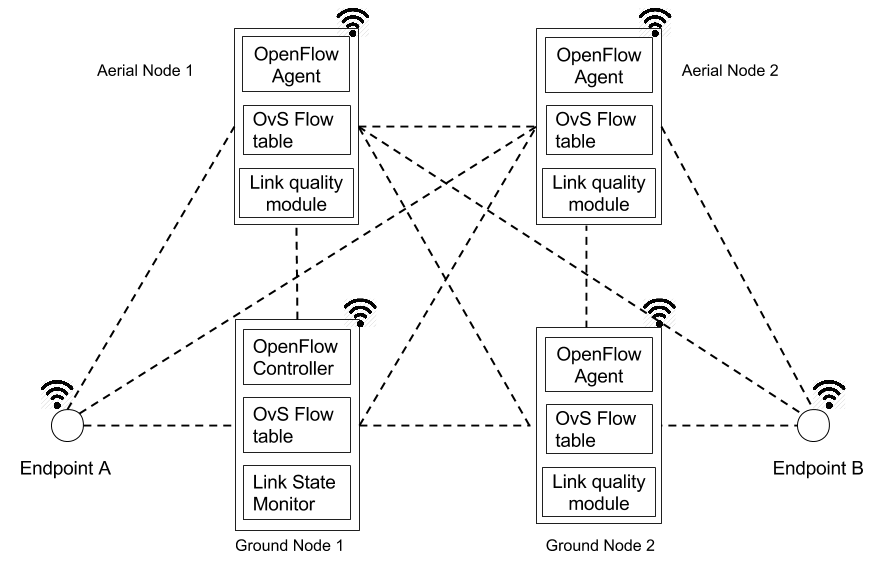
\includegraphics[width=\textwidth]{design}
\end{figure}
The above figure describes the overview of the components constituting this system. There exists a wireless ad-hoc
network of aerial and ground nodes. One of the nodes acts as an SDN controller and the others act as agents. A link
quality information (LQI) module is running on all the nodes in the network and this information is forwarded to the
OpenFlow controller which makes adaptive routing decisions. The controller will use this information to compute the
optimum end-to-end route between the endpoints. These routes will then be configured into the nodes using OpenFlow. The
nodes will have OpenFlow agent running on them which will configure the routes sent by the Controller. 
\subsection{Link Quality Information Module}
\begin{figure}[H]
\caption{Components in the Link Quality Information Module}
\centering
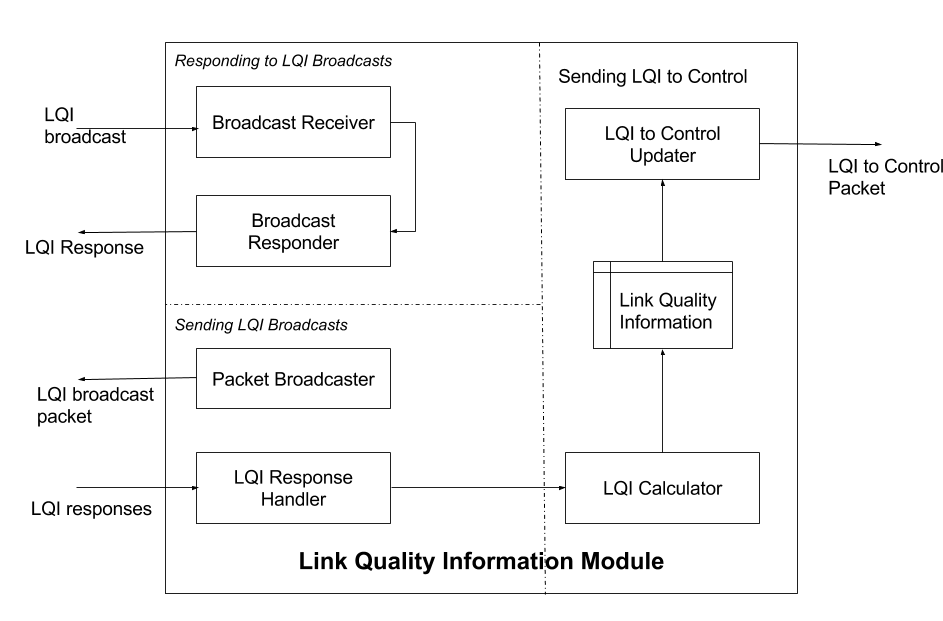
\includegraphics[width=\textwidth]{lqi}
\end{figure}
\noindent \textbf{Packet Broadcaster} \\
The packet broadcaster will broadcast packets at a regular interval to initiate the neighbour discovery. \\

\noindent \textbf{LQI Response Handler} \\
The LQI Response handler will wait for the responses to the broadcast packets sent by the Packet Broadcaster. It will
then forward these responses to the LQI calculator. \\

\noindent \textbf{Broadcast Receiver} \\
The broadcast receiver will receive the broadcast packets sent by the neighboring node LQI modules. \\

\noindent \textbf{Broadcast Responder} \\
Upon receiving the broadcast packets from the other LQI modules, the broadcast responder will send a response to the
appropriate nodes from where it received the broadcast packet. The response will be such that the other side will
appropriately be able to establish the link quality.\\

\noindent \textbf{LQI Calculator} \\
The LQI Calculator will assimilate all the responses from the neighbouring nodes and update the link quality information
table.\\

\noindent \textbf{LQI to Control Updater} \\
The LQI to Control Updater gets the calculated Link Quality Information from the LQI Calculator. It will send this
information over to the controller. \\
\subsection{OpenFlow Control Module}
\begin{figure}[H]
\caption{Components in the OpenFlow Control application}
\centering
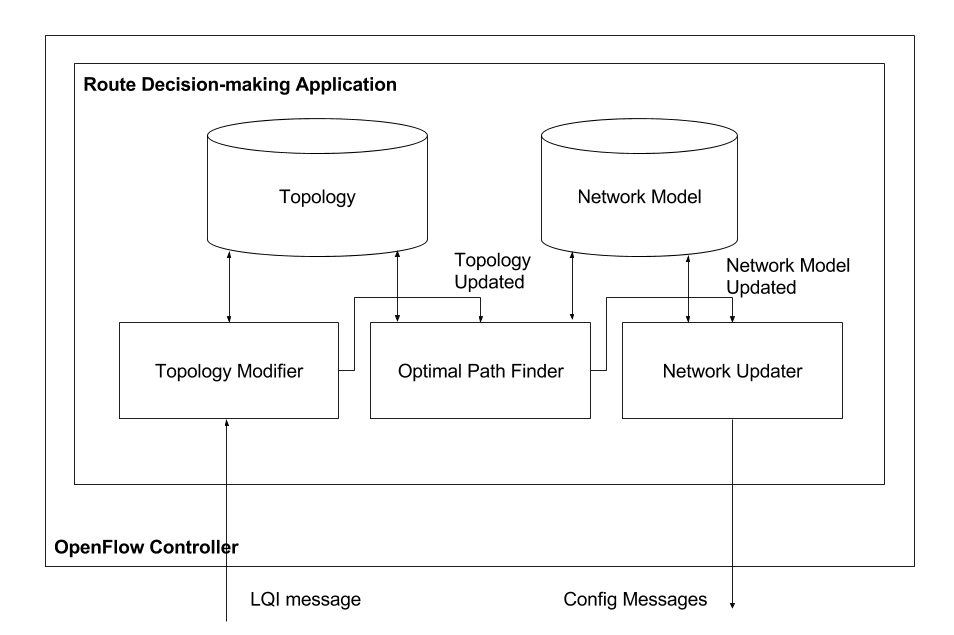
\includegraphics[width=\textwidth]{openflow}
\end{figure}
\noindent \textbf{Topology Modifier} \\
The LQI packets received by the controller will be send to this module to generate/update the network topology. The
topology will consists of the nodes and the link costs associated between each nodes. If there’s is a modification in
the topology, the Optimal Path Finder module will be notified to update the routes. \\

\noindent \textbf{Optimal Path Finder} \\
This module will keep a snapshot of the Network Model and compute the new model from the updated Topology. The new model
will be compared to the previous snapshot to detect changes. If the model has been modified, it will intimate the
Network Updater to configure these changes in Network.\\

\noindent \textbf{Network Updater} \\
If the Network Updater receives a call to configure the changes in the network, it will compute the changes from the
previous snapshot and then configure the routes that have been changed to appropriate nodes.
\section{Per-member Responsibilities}
\begin{tabular}{ | p{0.185\linewidth} | p{0.185\linewidth} | p{0.185\linewidth} | p{0.185\linewidth} | p{0.185\linewidth} | }
\hline
\textbf{Tasks}	&	\textbf{Angelyn Arputha Babu John}	&	\textbf{Jignesh Darji}	&	\textbf{Nishad Sabnis}	& \textbf{Alok Kulkarni} \\
\hline \hline
Node Setup	&	Implement	&	Implement	&	Implement	&	Implement \\
\hline
Creation of ad-hoc network	&	Review	&	Review	&	Implement	&	Implement \\
\hline
LQI Message Handling	&	Review	&	Review	&	Implement	&	Implement \\ 
\hline
LQI Calculator	&	Review	&	Review	&	Review	&	Implement\\ 
\hline
LQI to Control Updater	&	Review	&	Review	&	Implement	&	Review \\
\hline
Topology Modifier	&	Implement	&	Implement	&	Review	&	Review\\
\hline
Optimal Path Finder	&	Implement	&	Implement	&	Review	&	Review\\
\hline
Network Updater	&	Implement	&	Implement	&	Review	&	Review\\
\hline
\end{tabular}

\section{Timeline}
\begin{figure}[H]
\caption{Project Timeline}
\centering
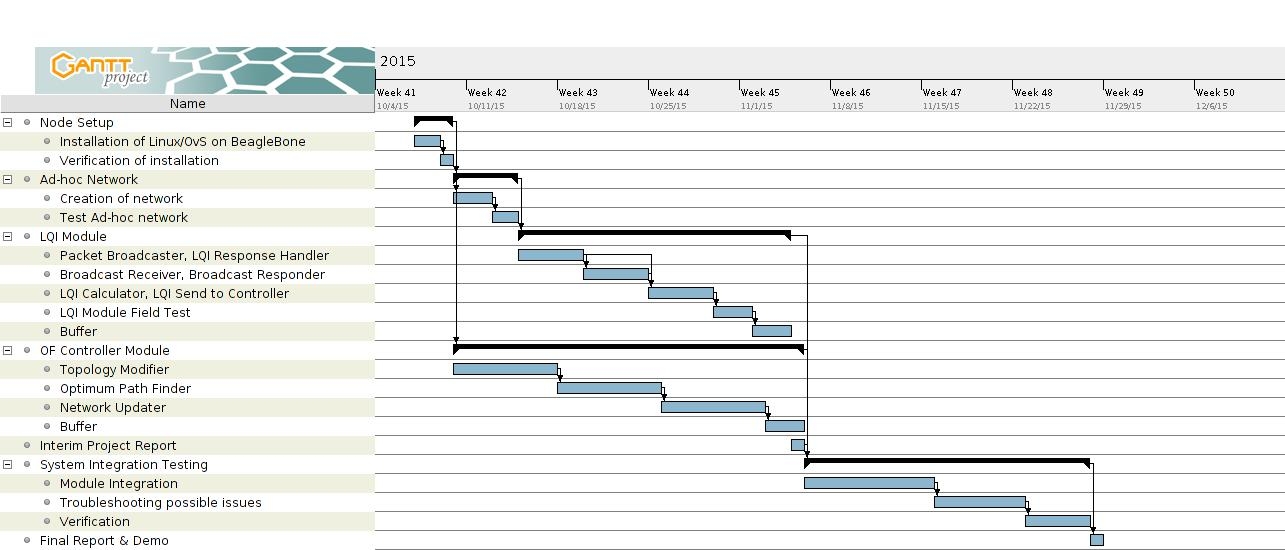
\includegraphics[width=\textwidth]{timeline}
\end{figure}

\begin{tabular}{  | p{.45\linewidth} | p{0.185\linewidth} | p{0.185\linewidth} | p{0.09\linewidth} |}
\hline
\textbf{Name}	&	\textbf{Begin date}	&	\textbf{End date}	&	\textbf{Duration (Days)} \\
\hline
Node Setup	&	10/7/15	&	10/9/15	&	3 \\
-Installation of Linux/OvS on BeagleBone	&	10/7/15	&	10/8/15	&	2 \\
-Verification of installation	&	10/9/15	&	10/9/15	&	1 \\
\hline
Ad-hoc Network	&	10/10/15	&	10/14/15	&	5 \\
-Creation of network	&	10/10/15	&	10/12/15	&	3 \\
-Test Ad-hoc network	&	10/13/15	&	10/14/15	&	2 \\
\hline
LQI Module	&	10/15/15	&	11/4/15	&	21 \\
-Packet Broadcaster, LQI Response Handler	&	10/15/15	&	10/19/15	&	5 \\
-Broadcast Receiver, Broadcast Responder	&	10/20/15	&	10/24/15	&	5 \\ 
-LQI Calculator, LQI Send to Controller	&	10/25/15	&	10/29/15	&	5 \\
-LQI Module Field Test	&	10/30/15	&	11/1/15	&	3 \\
-Buffer	&	11/2/15	&	11/4/15	&	3 \\
\hline
OF Controller Module	&	10/10/15	&	11/5/15	&	27 \\
-Topology Modifier	&	10/10/15	&	10/17/15	&	8 \\
-Optimum Path Finder	&	10/18/15	&	10/25/15	&	8 \\
-Network Updater	&	10/26/15	&	11/2/15	&	8 \\ 
-Buffer	&	11/3/15	&	11/5/15	&	3 \\
\hline
Interim Project Report	&	11/5/15	&	11/5/15	&	1 \\
\hline
System Integration Testing	&	11/6/15	&	11/27/15	&	22 \\
-Module Integration	&	11/6/15	&	11/15/15	&	10 \\
-Troubleshooting possible issues	&	11/16/15	&	11/22/15	&	7 \\
-Verification	&	11/23/15	&	11/27/15	&	5 \\
\hline
Final Report and Demo	&	11/28/15	&	11/28/15	&	1 \\
\hline
\end{tabular}

\section{Test Plan}
\begin{tabular}{  | p{0.185\linewidth} | p{0.185\linewidth} | p{0.185\linewidth} | p{0.185\linewidth} | p{0.185\linewidth} |}
\hline
\textbf{Test}	&	\textbf{LQI Module}	&	\textbf{Topology Modifier(TM)}	&	\textbf{Optimal Path Finder (OPF)}	&
\textbf{Network Updater(NU)}\\ 
\hline \hline
Add a node with low path cost	&	Connected nodes should transmit cost with the new node to the LQI messages	&	Add node to Topology; intimate OPF	&	Add to Network Model; intimate NU	&	Update affected nodes\\ 
\hline
Add a node with high path cost	&	Connected nodes should transmit cost with the new node to the LQI messages	&	Add node to Topology; intimate OPF	&	Network Model remains same	&	NA\\ 
\hline
Remove node from Network Model	&	LQI messages will not contain costs to this node	&	Remove node from Topology; intimate OPF	&	Modifies Network Model; intimate NU	&	Update affected nodes\\ 
\hline
Remove node not part of Network Model	&	LQI messages will not contain costs to this node	&	Remove node from Topology; intimate OPF	&	Network Model remains same	&	NA\\ 
\hline
Increase associated path cost of a node in Network Model	&	Cost to this node should be increased in the LQI messages	&	Update path costs in Topology; intimate OPF	&	Modifies Network Model; intimate NU	&	Update affected nodes\\ 
\hline
Increase associated path cost of a node NOT in Network Model	&	Cost to this node should be increased in the LQI messages	&	Update path costs in Topology; intimate OPF	&	Network Model remains same	&	NA\\ 
\hline
Decrease associated path cost of a node in Network Model	&	Cost to this node should be decreased in the LQI messages	&	Update path costs in Topology; intimate OPF	&	Network Model remains same	&	NA\\ 
\hline
Decrease associated path cost of a node NOT in Network Model	&	Cost to this node should be decreased in the LQI messages	&	Update path costs in Topology; intimate OPF	&	Modifies Network Model; intimate NU	&	Update affected nodes \\
\hline
\end{tabular}
\section{Demo Plan}
\begin{enumerate}
\item Once the ad-hoc network is setup, the controller will generate the Network Model and configure the rules in all
the nodes for the optimal path.
\item A display utility for the Network Model will print the current Network Model.
\item We'll display that these rules have been correctly configured in the nodes by connecting to each node and
displaying their rule tables.
\item Thus, on changing the distance between the nodes, we plan to show that the routes between the two endpoints change
dynamically based on the link strength. 
\end{enumerate}
\end{document}
